\documentclass[../main.tex]{subfiles}
\begin{document}

Chương này trình bày chi tiết các thực nghiệm để kiểm chứng độ chính xác của khung đo lường lý thuyết đã đề xuất ở Chương 2. Thông qua 11 tập dữ liệu toàn diện và 5 thuật toán phát hiện bất thường, nghiên cứu lần lượt phân tích bác bỏ giả định do phương pháp Marginal Overlap gây ra, xác lập sức mạnh giải thích của thước đo DensPct\_Mahal, giải thích cơ chế sụp đổ sớm F1-Score do hạn chế của AUC, và chứng minh tiềm năng cải thiện của phương pháp phi tham số (KDE\_Joint) cũng như chỉ ra các giới hạn của nó trước dữ liệu thưa thớt.

\section{Thiết lập thực nghiệm và cấu hình}
\label{section:3.1}

\subsection{Cấu hình hệ thống thực nghiệm}
Các thực nghiệm được tiến hành trên hệ thống máy trạm Windows 11, trang bị bộ vi xử lý AMD Ryzen 5 5600GT @ 3.3GHz (6 lõi, 12 luồng), RAM 16GB DDR5. Mã nguồn phân tích được triển khai trên môi trường Python 3.10.12, sử dụng các thư viện tính toán khoa học lõi bao gồm: NumPy 1.23.5, SciPy 1.10.1, và scikit-learn 1.2.2.

\subsection{Danh mục 11 tập dữ liệu thực nghiệm}
Thực nghiệm được triển khai trên 11 tập dữ liệu toàn diện bao gồm: 3 chiến dịch APT thực tế (BOTSv1, FIN6, APT29) và 8 kịch bản tấn công tổng hợp mô phỏng theo MITRE ATT\&CK được tạo ra bằng phương pháp Controlled Injection (KB1 đến KB8). Bảng \ref{tab:11datasets} tóm tắt số lượng tiến trình độc hại ($N$), mức độ chồng lấn phân phối biên trung bình DDO, và độ chui sâu trung tâm DensPct\_Mahal của các tập dữ liệu này:

\begin{table}[H]
\centering
\small
\setlength{\tabcolsep}{4pt}
\caption{Đặc tính cơ bản và độ khó của 11 tập dữ liệu nghiên cứu.}
\begin{tabular}{|p{2.2cm}|>{\centering\arraybackslash}p{2.2cm}|>{\centering\arraybackslash}p{1.8cm}|>{\centering\arraybackslash}p{2.8cm}|p{4.2cm}|}
\hline
\textbf{Tập dữ liệu} & \textbf{Số tiến trình độc hại ($N$)} & \textbf{DDO (mean)} & \textbf{DensPct\_Mahal (median)} & \textbf{Loại kịch bản} \\ \hline
\texttt{botsv1} & 3 & 0.5515 & 7.58\% & APT Thực tế \\ \hline
\texttt{fin6} & 31 & 0.6249 & 0.40\% & APT Thực tế \\ \hline
\texttt{apt29} & 22 & 0.6453 & 26.98\% & APT Thực tế \\ \hline
\texttt{kb1\_macro} & 3 & 0.6319 & 0.00\% & Controlled Injection \\ \hline
\texttt{kb2\_fileless} & 2 & 0.4849 & 4.03\% & Controlled Injection \\ \hline
\texttt{kb3\_wmiburst} & 8 & 0.6249 & 0.00\% & Controlled Injection \\ \hline
\texttt{kb4\_inject} & 2 & 0.6239 & 0.00\% & Controlled Injection \\ \hline
\texttt{kb5\_slow} & 4 & 0.6197 & 2.27\% & Controlled Injection \\ \hline
\texttt{kb6\_recon} & 25 & 0.7074 & 10.64\% & Controlled Injection \\ \hline
\texttt{kb7\_ransom} & 18 & 0.6991 & 2.04\% & Controlled Injection \\ \hline
\texttt{kb8\_lateral} & 51 & 0.6748 & 0.00\% & Controlled Injection \\ \hline
\end{tabular}
\label{tab:11datasets}
\end{table}

\subsection{Phương pháp chọn ngưỡng (Threshold Protocol)}
Để thiết lập giới hạn trên lý thuyết (theoretical upper bound) về hiệu năng phân tách của các thuật toán, luận văn sử dụng phương pháp \textbf{Optimal Oracle Threshold} — tức là ngưỡng được tối ưu hóa trực tiếp trên toàn bộ tập dữ liệu để đạt giá trị F1 lớn nhất. Việc áp dụng Optimal Oracle Threshold ở đây hoàn toàn không nhằm mục đích đề xuất một mô hình triển khai thực tiễn. Thay vào đó, việc áp dụng cơ chế Oracle \textbf{đồng nhất cho tất cả các thuật toán} (iForest, ECOD, LOF, KDE\_Joint) tạo ra một sân chơi công bằng tuyệt đối (Level Playing Field). Bằng cách loại bỏ biến nhiễu từ các chiến lược tự động chọn ngưỡng, Oracle Threshold cô lập và phản ánh chính xác \textbf{năng lực phân tách phân phối nội tại} (distributional separability) của từng mô hình.

\begin{table}[H]
\centering
\renewcommand{\arraystretch}{1.3}
\setlength{\tabcolsep}{3.0pt}
\small
\caption{Hiệu năng với Optimal Threshold trên 11 tập dữ liệu (đã loại trừ \texttt{apt3}). Bảng trình bày F1 (kèm Độ phủ/Recall trong ngoặc) và AUC.}
\begin{tabular}{@{}l|cc|cc|cc|cc|cc@{}}
\toprule
\multirow{2}{*}{\textbf{Tập dữ liệu}} & \multicolumn{2}{c|}{\textbf{iForest}} & \multicolumn{2}{c|}{\textbf{ECOD}} & \multicolumn{2}{c|}{\textbf{LOF}} & \multicolumn{2}{c|}{\textbf{SRAH}} & \multicolumn{2}{c}{\textbf{KDE\_Joint}} \\ \cmidrule(l){2-11} 
 & \textbf{F1 (Rec)} & \textbf{AUC} & \textbf{F1 (Rec)} & \textbf{AUC} & \textbf{F1 (Rec)} & \textbf{AUC} & \textbf{F1 (Rec)} & \textbf{AUC} & \textbf{F1 (Rec)} & \textbf{AUC} \\ \midrule
\texttt{botsv1} & 0.412 (1.00) & 0.870 & 0.429 (1.00) & 0.879 & 0.286 (1.00) & 0.773 & 0.500 (0.66) & 0.929 & 1.000 (1.00) & 1.000 \\
\texttt{fin6} & 0.314 (0.52) & 0.964 & 0.480 (0.38) & 0.959 & 0.348 (0.38) & 0.981 & 0.612 (0.83) & 0.915 & 0.967 (0.93) & 0.999 \\
\texttt{apt29} & 0.336 (0.30) & 0.773 & 0.368 (0.31) & 0.623 & 0.137 (0.50) & 0.576 & 0.345 (0.22) & 0.666 & 0.778 (0.63) & 0.958 \\
\texttt{kb1\_macro} & 0.500 (0.33) & 0.955 & 0.400 (0.66) & 0.931 & 0.500 (0.33) & 0.942 & 0.800 (0.66) & 0.676 & 1.000 (1.00) & 1.000 \\
\texttt{kb2\_fileless} & 0.667 (0.50) & 0.951 & 0.667 (0.50) & 0.955 & 0.182 (1.00) & 0.881 & 1.000 (1.00) & 1.000 & 0.667 (0.50) & 0.980 \\
\texttt{kb3\_wmiburst} & 0.508 (1.00) & 0.897 & 0.444 (1.00) & 0.905 & 0.769 (0.62) & 0.983 & 0.571 (1.00) & 0.928 & 1.000 (1.00) & 1.000 \\
\texttt{kb4\_inject} & 0.600 (0.50) & 0.952 & 0.286 (0.50) & 0.926 & 0.667 (0.50) & 0.937 & 0.400 (1.00) & 0.958 & 1.000 (1.00) & 1.000 \\
\texttt{kb5\_slow} & 0.447 (1.00) & 0.946 & 0.462 (0.75) & 0.942 & 0.320 (1.00) & 0.902 & 0.600 (0.75) & 0.957 & 0.857 (0.75) & 0.991 \\
\texttt{kb6\_recon} & 0.725 (1.00) & 0.899 & 0.725 (1.00) & 0.879 & 0.746 (1.00) & 0.901 & 0.359 (0.28) & 0.303 & 0.725 (1.00) & 0.924 \\
\texttt{kb7\_ransom} & 0.773 (1.00) & 0.937 & 0.655 (1.00) & 0.885 & 0.679 (1.00) & 0.925 & 0.780 (0.88) & 0.871 & 0.839 (0.72) & 0.991 \\
\texttt{kb8\_lateral} & 0.843 (1.00) & 0.884 & 0.843 (1.00) & 0.884 & 0.909 (0.98) & 0.952 & 0.675 (0.51) & 0.510 & 1.000 (1.00) & 1.000 \\
\bottomrule
\end{tabular}
\label{tab:3.2}
\end{table}

\section{Bác bỏ giả định DDO (Phân tích Scatter plot)}
\label{section:3.2}

Đại lượng DDO (Degree of Distribution Overlap) đo lường mức độ chồng lấn phân phối của các đặc trưng trên các biên đơn chiều độc lập. Từng được xem là tiêu chuẩn dự đoán độ khó, kết quả thực nghiệm chỉ ra sự thiếu tương quan nghiêm trọng giữa DDO và hiệu năng phát hiện.

\begin{figure}[H]
\centering
\begin{tikzpicture}
\begin{axis}[
    xlabel={Marginal Overlap (DDO\_mean)},
    ylabel={AUC Score (LOF)},
    xmin=0.4, xmax=0.8,
    ymin=0.5, ymax=1.05,
    width=0.8\textwidth,
    height=0.45\textwidth,
    title={Spearman $\rho = 0.251, p = 0.46$}
]
\addplot[only marks, mark=*, red] table {
x y
0.5515 0.7273
0.6249 0.9858
0.6453 0.5709
0.6319 0.9514
0.4849 0.8842
0.6249 0.9975
0.6239 0.9754
0.6197 0.9669
0.7074 0.9261
0.6991 0.9854
0.6748 0.9981
};
\node[below, font=\scriptsize] at (axis cs:0.5515, 0.7273) {botsv1};
\node[above, font=\scriptsize] at (axis cs:0.6249, 0.9858) {fin6};
\node[below, font=\scriptsize] at (axis cs:0.6453, 0.5709) {apt29};
\node[below, font=\scriptsize] at (axis cs:0.4849, 0.8842) {kb2};
\node[left, font=\scriptsize, align=right] at (axis cs:0.68, 0.92) {Cụm tổng hợp\\(KB1, KB3-KB8)};
\end{axis}
\end{tikzpicture}
\caption{Biểu đồ tán xạ giữa DDO và AUC. Sự phân tán vô trật tự bác bỏ mối tương quan giữa độ chồng lấn biên và hiệu năng.}
\label{fig:3.1}
\end{figure}

Phân tích số liệu cho thấy, rất nhiều kịch bản tấn công sở hữu mức độ chồng lấn biên cực kỳ cao như \texttt{kb6\_recon} (DDO = 0.707) hay \texttt{kb8\_lateral} (DDO = 0.675). Theo logic thông thường, các tập này phải rất khó phát hiện do hành vi của mã độc hòa trộn mạnh. Tuy nhiên, thuật toán LOF vẫn đạt mức F1 và AUC rất cao. \textit{(LOF được cấu hình sử dụng khoảng cách Gower thông qua phép chiếu Manhattan để đo lường công bằng trên không gian V10)}.

Kiểm định tương quan hạng Spearman giữa DDO và AUC chỉ đạt mức $\rho = 0.251$ với giá trị $p-value = 0.46$. Do $p > 0.05$, không có ý nghĩa thống kê để kết luận DDO có khả năng dự đoán hiệu năng. Kết quả này chính thức bác bỏ giả định ngây thơ về độ chồng lấn biên, chứng minh hiện tượng **Marginal Blindness** tạo ra sự nhầm lẫn về mức độ ngụy trang.

\section{Sức mạnh giải thích của BBS}
\label{section:3.3}

Trái ngược với DDO, thước đo cấu trúc toàn cục DensPct\_Mahal thể hiện năng lực giải thích vượt trội đối với hiệu năng của hệ thống.

\begin{figure}[H]
\centering
\begin{tikzpicture}
\begin{axis}[
    xlabel={Global Depth (DensPct\_median \%)},
    ylabel={AUC Score (LOF)},
    xmin=-5, xmax=35,
    ymin=0.5, ymax=1.05,
    width=0.8\textwidth,
    height=0.45\textwidth,
    title={Spearman $\rho = -0.796, p = 0.003$}
]
\addplot[only marks, mark=*, blue] table {
x y
7.58 0.7273
0.4 0.9858
26.98 0.5709
0.0 0.9514
4.03 0.8842
0.0 0.9975
0.0 0.9754
2.27 0.9669
10.64 0.9261
2.04 0.9854
0.0 0.9981
};
\addplot [thick, red, dashed, domain=-2:30] {-0.0125*x + 0.98};
\node[below, font=\scriptsize] at (axis cs:7.58, 0.7273) {botsv1};
\node[right, font=\scriptsize] at (axis cs:0.4, 0.9858) {fin6};
\node[below, font=\scriptsize] at (axis cs:26.98, 0.5709) {apt29};
\node[right, font=\scriptsize] at (axis cs:10.64, 0.9261) {kb6};
\node[right, font=\scriptsize] at (axis cs:4.03, 0.8842) {kb2};
\node[left, font=\scriptsize, align=right] at (axis cs:-1, 0.98) {Cụm KB\\(Độ sâu 0\%)};
\end{axis}
\end{tikzpicture}
\caption{Biểu đồ DensPct\_Mahal và AUC. Sự tương quan nghịch đảo rõ rệt minh chứng cho hiện tượng Sụp đổ sớm (Early Collapse).}
\label{fig:3.2}
\end{figure}

Kiểm định hoán vị (Permutation Test) với 10,000 vòng lặp xác nhận giá trị $p-value = 0.0077$, nhỏ hơn mức ý nghĩa $\alpha = 0.01$. Bằng chứng này khẳng định mối liên hệ thống kê giữa việc mã độc chui sâu vào trung tâm (DensPct\_Mahal lớn) và sự suy giảm hiệu năng thuật toán.

\subsection{Phân tích nhạy Leave-One-Out}
Để kiểm chứng kết quả Spearman không bị chi phối bởi các điểm đòn bẩy, phân tích Leave-One-Out được thực hiện (loại bỏ từng tập và tính lại $\rho$). Kết quả cho thấy khi loại bỏ tập ảnh hưởng mạnh nhất là \texttt{apt29}, tương quan nghịch vẫn duy trì ý nghĩa thống kê ($p = 0.017 < 0.05$). Điều này chứng minh mối quan hệ giữa DensPct\_Mahal và AUC là ổn định (robust).

\subsection{Hiện tượng sụp đổ sớm F1-Score do hạn chế của AUC}
Quan sát kỹ, ngay cả khi DensPct\_Mahal tăng lên 26.98\% (tập \texttt{apt29}), AUC vẫn ở mức $0.5709$ (tốt hơn đoán ngẫu nhiên). Tuy nhiên, trong thực tế nơi dữ liệu log mất cân bằng cực đoan, AUC tạo ra **ảo giác hiệu năng**. Đánh giá bằng **F1-Score** bộc lộ hiện tượng **Sụp đổ sớm (Early Collapse)**: chỉ cần mã độc hòa trộn cấu trúc rất nhỏ ($DensPct \approx 2\% - 7\%$), các thuật toán UAD truyền thống đã mất khả năng phân tách (F1 sụp xuống dưới 0.37). Kẻ tấn công không cần hòa trộn hoàn toàn để vô hiệu hóa hệ thống, củng cố lý thuyết về **Global Center Bias**.

\section{Phá vỡ giới hạn bằng Bằng chứng tồn tại (KDE\_Joint)}
\label{section:3.4}

Để chứng minh sự sụp đổ hiệu năng tại $DensPct = 27\%$ trên tập \texttt{apt29} không phải là ngõ cụt kỹ thuật, mô hình phi tham số KDE\_Joint được áp dụng như một minh chứng tồn tại (Existence Proof).

\begin{figure}[H]
\centering
\begin{tikzpicture}
\begin{axis}
[
    ybar,
    enlargelimits=0.15,
    legend style={at={(0.5,-0.15)}, anchor=north,legend columns=-1},
    ylabel={F1-Score},
    symbolic x coords={LOF, iForest, ECOD, SRAH, KDE\_Joint (Semi)},
    xtick=data,
    nodes near coords,
    nodes near coords align={vertical},
    width=0.8\textwidth,
    height=0.45\textwidth,
    title={Bằng chứng tồn tại: Hiệu năng F1-Score trên tập dữ liệu APT29}
]
\addplot[fill=red!60] coordinates {(LOF,0.103) (iForest,0.336) (ECOD,0.368) (SRAH,0.345)};
\addplot[fill=green!60] coordinates {(KDE\_Joint (Semi),0.778)};
\legend{Mô hình biên (Marginal Bias), Phi tham số (Local Pockets)}
\end{axis}
\end{tikzpicture}
\caption{Biểu đồ so sánh F1-Score trên tập dữ liệu APT29. KDE\_Joint cải thiện đáng kể hiệu năng.}
\label{fig:3.3}
\end{figure}

Trong khi các thuật toán mang thiên kiến toàn cục sụp đổ (F1 $< 0.37$), KDE\_Joint đạt mức **F1 = 0.778** (tăng 125\% so với SRAH). Điều này chứng minh hành vi ngụy trang của APT29 không vô hình, mà chỉ bị che khuất bởi các giả định hình học. Bằng cách khai thác mật độ đồng thời phi tham số trên không gian hỗn hợp V10, KDE\_Joint định vị thành công các **Local Pockets** mà mã độc đang lẩn trốn.

\begin{figure}[H]
\centering
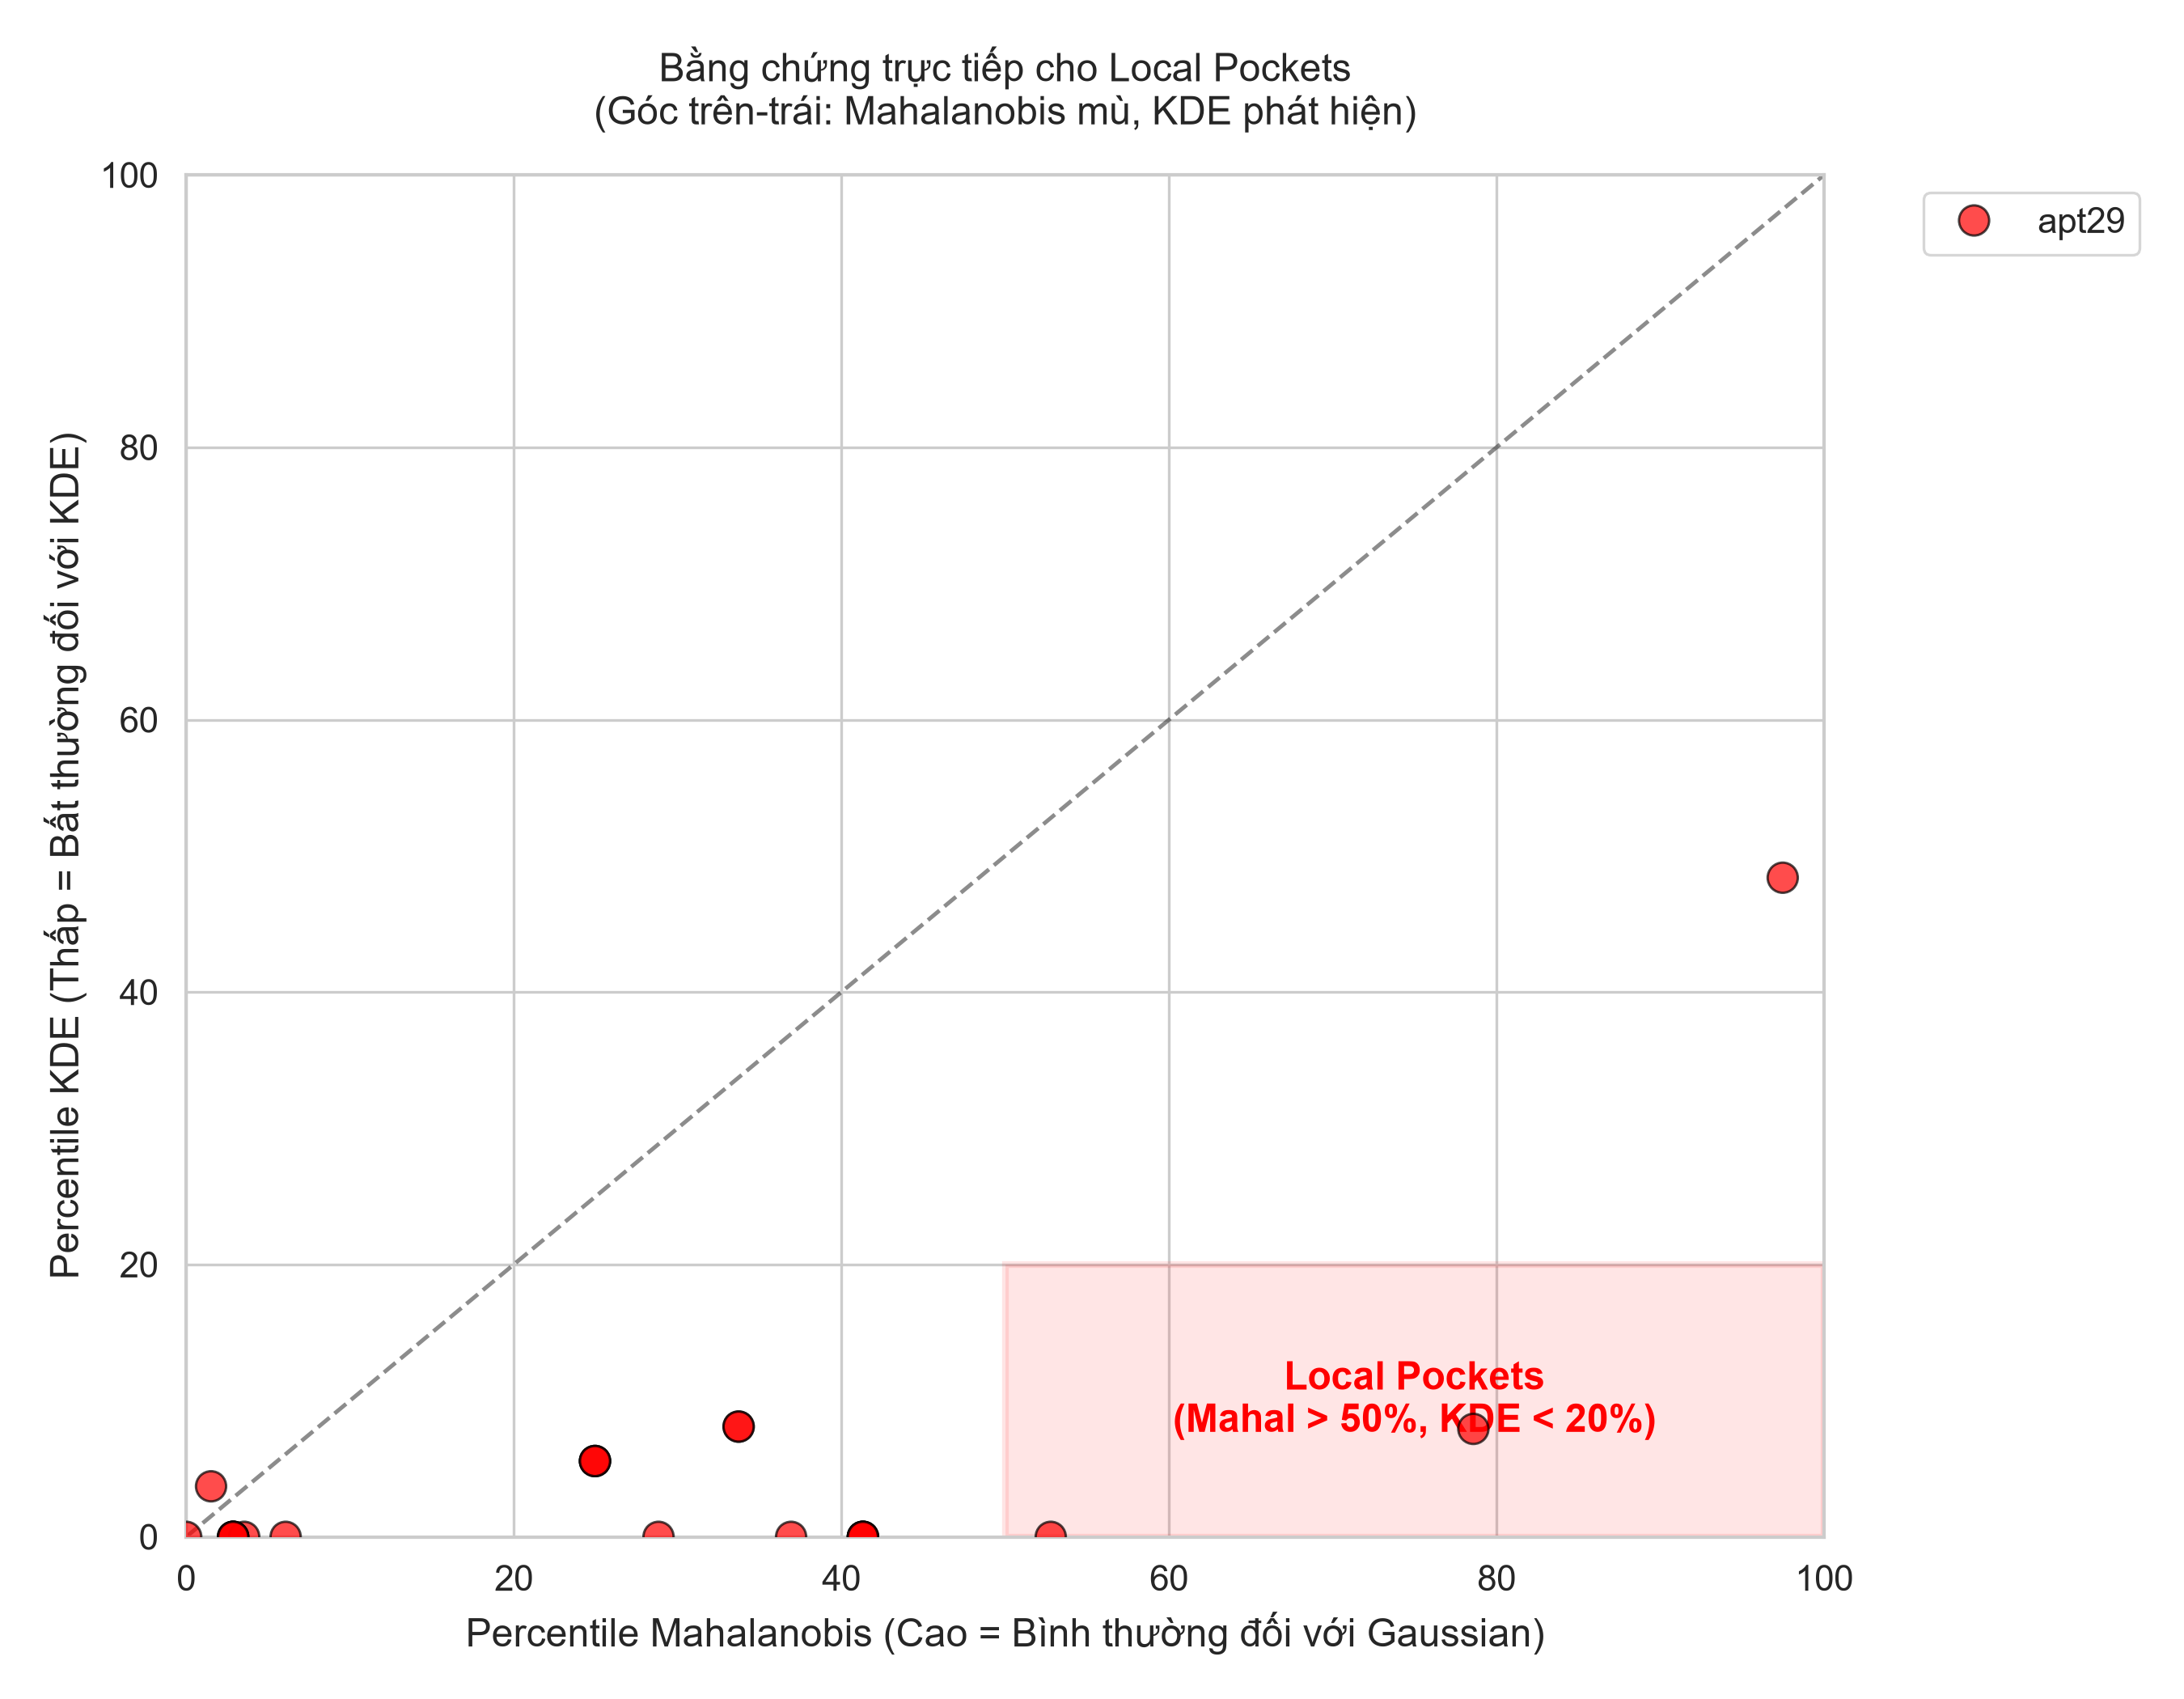
\includegraphics[width=0.85\textwidth]{../images/fig_hero_local_pockets.png}
\caption{Đối chiếu Mahalanobis Percentile và KDE Percentile. Các tiến trình APT29 (màu đỏ) tập trung tại góc trên-trái (Gaussian đánh giá an toàn, KDE đánh giá bất thường), cung cấp minh chứng trực quan cho sự tồn tại của Local Pockets.}
\label{fig:hero_local_pockets}
\end{figure}

\section{Giới hạn và Failure Mode của phân tích cấu trúc cục bộ}
\label{section:3.5}

Mặc dù KDE\_Joint là công cụ lý thuyết mạnh mẽ, nó đối mặt với giới hạn lớn trong môi trường thực tế (SOC) do độ phức tạp suy diễn $O(N^2 \cdot d)$. Hơn nữa, thuật toán bộc lộ cơ chế lỗi (Failure Mode) nghiêm trọng trên không gian đặc trưng thưa thớt (như tập \texttt{kb8\_lateral}).

Thuộc tính phân loại thưa thớt khiến tham số bandwidth ($h$) bị đánh giá quá nhỏ (\textit{underestimation}), dẫn đến hàm mật độ tại điểm kiểm thử bị thoái hóa về 0 (log-likelihood = $-\infty$). Mô hình hoàn toàn mất khả năng thiết lập ngưỡng phân tách. Trái lại, thước đo DensPct\_Mahal vẫn ổn định nhờ tính kháng nhiễu của hiệp phương sai toàn cục. Phát hiện này đặt ra bài toán tương lai: thiết kế bộ ước lượng mật độ lai ghép (hybrid estimator) tận dụng độ ổn định của Mahalanobis và độ nhạy của KDE.

\end{document}
